%        File: 
%     Created: Tue 07:06, 3 May 2022
% Last Change: Thu 03:39, 5 May 2022
%
% \documentclass[a4paper, 10pt]{article}
\documentclass[a4paper, 10pt]{report}


\usepackage[general]{fancymath}
\usepackage{fancycom}
\usepackage[colorlinks]{hyperref}
\usepackage{subcaption}

\usepackage[export]{adjustbox}

\usepackage{dirtree}
\usepackage{fontawesome}

\usepackage{multicol}
\usepackage{multirow}

\usepackage{bera}% optional: just to have a nice mono-spaced font
\usepackage{listings}

\usepackage{longtable}

\makeatletter
\newcommand{\groupedRowColors}[5][0]{% [#1: offset], #2: group size, #3: start line, #4: color 1, #5: color 2
    % copied from xcolor.sty
    \global\rownum=\z@
    \global\@rowcolorstrue
    \@ifxempty{#4}%
        {\def\@oddrowcolor{\@norowcolor}}%
        {\def\@oddrowcolor{\gdef\CT@row@color{\CT@color{#4}}}}%
    \@ifxempty{#5}%
        {\def\@evenrowcolor{\@norowcolor}}%
        {\def\@evenrowcolor{\gdef\CT@row@color{\CT@color{#5}}}}%
    % simplified (no check for \if@rowcmd)
    \def\@rowcolors{%
        \if@rowcolors
            \noalign{%
                \relax
                \ifnum\rownum<#3
                    \@norowcolor
                % I have changed this check:
                \else \ifodd \numexpr (\rownum-#1)/#2\relax
                    \@oddrowcolor
                \else
                    \@evenrowcolor
                \fi \fi
            }%
        \fi
    }%
    \CT@everycr{\@rowc@lors\the\everycr}%
    \ignorespaces
}
\makeatother

\definecolor{eclipseStrings}{RGB}{42,0.0,255}
\definecolor{eclipseKeywords}{RGB}{127,0,85}
\colorlet{numb}{magenta!60!black}

\lstdefinelanguage{json}{
    basicstyle=\normalfont\ttfamily,
    commentstyle=\color{eclipseStrings}, % style of comment
    stringstyle=\color{eclipseKeywords}, % style of strings
    numbers=left,
    numberstyle=\scriptsize,
    stepnumber=1,
    numbersep=8pt,
    showstringspaces=false,
    breaklines=true,
    frame=lines,
    string=[s]{"}{"},
    comment=[l]{:\ "},
    morecomment=[l]{:"},
    escapechar=|,
    literate=
        *{0}{{{\color{numb}0}}}{1}
         {1}{{{\color{numb}1}}}{1}
         {2}{{{\color{numb}2}}}{1}
         {3}{{{\color{numb}3}}}{1}
         {4}{{{\color{numb}4}}}{1}
         {5}{{{\color{numb}5}}}{1}
         {6}{{{\color{numb}6}}}{1}
         {7}{{{\color{numb}7}}}{1}
         {8}{{{\color{numb}8}}}{1}
         {9}{{{\color{numb}9}}}{1}
}

\newcommand{\FTdir}{}
\def\FTdir(#1,#2,#3){%
  \FTfile(#1,{{\color{black!40!white}\faFolderOpen}\hspace{0.2em}#3})
  (tmp.west)++(0.8em,-0.4em)node(#2){}
  (tmp.west)++(1.5em,0)
  ++(0,-1.3em) 
}

\newcommand{\FTfile}{}
\def\FTfile(#1,#2){%
  node(tmp){}
  (#1|-tmp)++(0.6em,0)
  node(tmp)[anchor=west,black]{\tt #2}
  (#1)|-(tmp.west)
  ++(0,-1.2em) 
}

\def\FTfileicon(#1,#2,#3){%
  \FTfile(#1,{{\color{black!40!white}#2}\hspace{0.2em}#3})
}

\def\FTimage(#1,#2){%
  \FTfileicon(#1,\faFilePictureO,#2)
}

\newcommand{\FTroot}{}
\def\FTroot{tmp.west}

\aname{Conatum}
\stitle{StudyLion GUI Skin Data Specification}

\begin{document}
\tableofcontents
\setcounter{chapter}{-1}
\chapter{Introduction}
This is a work-in-progress specification of the StudyLion GUI skinning interface.

This specification is mainly intended to be used as a reference guide while creating or modifying
global skins for StudyLion.

The suggested way to read this specification is start from the appendix, wherein there is a worked example
of a complete skin (the actual StudyLion Obsidian skin data).
The properties and assets of this example link back to tabulated descriptions in the text itself for more information.

The example skin may also be found on the skins plugin Github repository, and used as a template if desired.

In its present state, the specification is still highly incomplete as a full guide to skin properties and customisation.
However, it should describe all relevant properties needed for basic skin creation,
where assets are replaced with equivalent ones, and only colour properties need modification.
\chapter{\texttt{skin.json} File Structure}
\section{Template}
\begin{lstlisting}[language=json,firstnumber=1]
{
  "display_name": "Sample Skin",
  "description": "A sample skin template",
  "public": true,
  "price": 1024,
  "asset_root": "assets",
  "parents": ["base"],
  "guild_whitelist": [917704915311276032],
  "user_whitelist": [514205586502713365],
  "properties": {
    "common": {
    },
    "tasklist": {
    },
    "stats": {
    },
    "profile": {
    },
    "weekly_stats": {
    },
    "monthly_stats": {
    },
    "weekly_goals": {
    },
    "monthly_goals": {
    },
    "leaderboard": {
    }
  }
}
\end{lstlisting}
\section{Description}
The \texttt{skin.json} file goes in the skin \emph{root} directory (e.g. \texttt{skins/obsidian/skin.json}),
and describes the skin metadata (e.g. the visible name, price, asset location, etc),
as well as any \emph{card properties} that this skin specifies (i.e. colours, spaces, strings, etc).
\section{Fields}
\emph{All} fields except \texttt{properties} are optional, however most fields should be provided for visible skins
(i.e. skins that will be visible to at least one regular user).
\renewcommand{\arraystretch}{1.2}
\rowcolors{1}{Tan}{Apricot}
\begin{longtable}{| p{.15\textwidth} p{.85\textwidth} |}
  \hline
  \rowcolor{gray}
  Field & Description \\ \hline \endfirsthead
  \texttt{display\_name} &
  \textbf{Required} for visible skins.\newline
  \textbf{Type:} A string less than \texttt{25} characters.\newline
  \textbf{Default:} \texttt{"Unnamed"} \newline
  The name of skin displayed to users in selection menus and any configuration.\newline
  May be changed without notice (unlike the \texttt{skin\_id} in the \texttt{skins.json} file).
  \\
  \texttt{description} &
  \textbf{Required} for visible skins.\newline
  \textbf{Type:} A string less than \texttt{100} characters.\newline
  The description users will see for this skin in selection menus.
  \\
  \texttt{public} &
  \textbf{Optional.}\newline
  \textbf{Type:} Either \texttt{true} or \texttt{false}.\newline
  \textbf{Default:} \texttt{false}\newline
  Whether this is a \emph{public} skin, visible to any guild or user who can access a skin shop or selection menu.\newline
  This explicitly overrides \texttt{guild\_whitelist} and \texttt{user\_whitelist}.
  \\
  \texttt{price} &
  \textbf{Optional.}\newline
  \textbf{Type:} Any integer.\newline
  \textbf{Default:} \texttt{0}\newline
  The number of LionGems this skin costs in the premium user skin shops.
  \\
  \texttt{asset\_root} &
  \textbf{Optional.} But \textbf{Required} for any skins with custom assets.\newline
  \textbf{Type:} A \emph{folder path} relative to the skin directory.\newline
  \textbf{Default:} No value.\newline
  The relative path to search for assets for this skin.

  For example, if the skin directory is \texttt{skins/obsidian} and \texttt{asset\_root}
  is \texttt{"assets"}, then assets will be searched under \texttt{skins/obsidian/assets}.

  If this value is \emph{not} provided, the skin directory will not be searched for assets.
  \\
  \texttt{PATH} &
  \textbf{Optional.} Generally not required.\newline
  \textbf{Type:} A list of folder paths relative to the skin directory.\newline
  \textbf{Default:} No value.\newline
  Extra paths to search for assets, similar to \texttt{asset\_root}.
  These will be searched in \emph{descending} order, so assets found in the end of the \texttt{PATH}
  will be used before assets found in the start of the \texttt{PATH}.

  \texttt{asset\_root} will always be searched \emph{first}, if provided.
  \\
  \texttt{parents} &
  \textbf{Required} for usable skins. \textbf{Optional} for abstract skins. \newline
  \textbf{Type:} A list of \texttt{skin\_id}'s, as specified in the top-level \texttt{skins.json}. \newline
  \textbf{Default:} No value.\newline
  A list of skins that this skin should \emph{inherit} its card properties and assets from.
  If an asset or property is not found in this skin, the \emph{parent} skins will be searched,
  with the last provided skin being searched first.
  This allows for a collection of skins to share a common set of default properties or assets (given in a shared parent).

  All usable skins should inherit from \texttt{base}, as this skin provides the common masks and other default assets.

  Abstract skins (only intended to be used as shared parents to provide a common collection of defaults),
  generally should not inherit from \texttt{base}.
  \\
  \texttt{properties} &
  \textbf{Required.} All skins must have this field, although it may be empty.\newline
  This is a map of \texttt{card\_id -> card\_properties}.\newline
  See Chapter \ref{chapter:cards} for a detailed description of available card properties.\newline
  All cards and properties are \emph{optional}, and if given will override any values provided in the parents, or the default.
  This includes colour codes, asset paths, and spaces.
  These properties are not required to actually exist on the card, so beware of typos!\newline
  The special card id \texttt{"common"}, if given, specifies common values for \emph{all} cards.
  \\
  \hline
\end{longtable}

\section{A note on Card Inheritance}
\section{A note on Skin Inheritance}
\chapter{Cards}\label{chapter:cards}
\section{Structure}
A card skin is comprised of \emph{properties}, described in the \texttt{skin.json} file,
and \emph{assets}, which are images placed in the \hyperlink{skin-asset-root}{\texttt{"asset-root"}}
used either directly as components of the card (e.g. the background),
or as masks describing information \emph{about} components of the card.

\emph{All} properties and assets are optional, and if not provided, will default to the values in the base skin
(see also the \hyperlink{skin-parents}{\texttt{"parents"}} field of the \texttt{skin.json} file.).
Thus, a skin only needs to provide the properties and assets which it needs to \emph{change} from the default values.

This chapter will describe the modifiable properties and assets of each card in detail,
and attempt to display where they appear on the rendered card and what requirements they have in a skin.

As usual, please see the Appendix for a complete annotated skin example,
where each asset and property is hyperlinked back to the detailed descriptions in this chapter.
\subsection{Properties}
The following types of properties may be customised for each card.
\begin{itemize}
  \item \emph{Colour Properties}. These are colours for various components of the card, and should be specified
    as either RGB or RGBA hex values, e.g. \texttt{"\#A3A5F3"} or \texttt{"\#A3A5F380"},
    with the latter describing an alpha channel value of $128$ out of $256$, and hence $50\%$ opacity.

    In the below specification, each colour property is given with its key (for the \texttt{skin.json} file),
    a brief description, and an "In Context" card which is typically the default version of the card rendered with sample arguments,
    where the colour has been replaced with a highlight colour (usually some shade of red).
  \item \emph{Asset Paths}. Each included \emph{asset} lives at a particular location.

    When including an asset in a skin, it should usually be placed at its \emph{default path},
    that is, the path of the asset in the default skin.

    However, this path may be customised in the \texttt{skin.json} file
    by giving the new path (relative to the \texttt{"asset\_root"}) as a value to the \emph{asset path key}.
    This is useful in several cases, e.g. to avoid duplicating assets which are the same in the new skin,
    but have different default paths.

    In the below specification, each \emph{Asset} is shown with a brief description, its specific requirements,
    the default image, default path, and default size. New assets should generally match the default size wherever possible,
    but most assets (not including masks!) allow some variability.

    If a new path is \emph{not} specified in the \texttt{skin.json} file,
    any new assets should be placed in relative \texttt{default path} stated in the properties.
  \item \emph{Spacing Properties}.
    In some cases it is desirable for a skin to have a slightly different layout than usual, perhaps to accommodate
    a differently sized asset (e.g. a new avatar border, or custom ends on the profile badges), or simply to provide a new appearance.

    In this case, there are many spacing properties that may be overridden to fine-tune the gaps and separators in the rendered card.

    \emph{To be completed -- these properties are available, but I haven't written the specification for them yet.}
\end{itemize}

\section{Tasklist}
\subsection{Colour Properties}
\rowcolors{1}{Tan}{Apricot}
\begin{longtable}{| p{.35\textwidth} p{.40\textwidth} p{.25\textwidth} |}
  \hline
  \rowcolor{gray}
  Property key & Description & In Context \\ \hline \endhead
  \hypertarget{tasklist-title-colour}{\texttt{title\_colour}} & Colour of the first page card title. &
  \includegraphics[width=.25\textwidth,valign=m]{images/tasklist/title_colour.png}
  \\
  \hypertarget{tasklist-mini-profile-name-colour}{\texttt{mini\_profile\_name\_colour}} & Colour of the user name on the first page profile. &
  \includegraphics[width=.25\textwidth,valign=m]{images/tasklist/mini_profile_name_colour.png}
  \\
  \hypertarget{tasklist-mini-profile-discrim-colour}{\texttt{mini\_profile\_discrim\_colour}} & Colour of the discriminator on the first page profile. &
  \includegraphics[width=.25\textwidth,valign=m]{images/tasklist/mini_profile_discrim_colour.png}
  \\
  \hypertarget{tasklist-mini-profile-badge-colour}{\texttt{mini\_profile\_badge\_colour}} & Colour of the badge background on the first page profile. &
  \includegraphics[width=.25\textwidth,valign=m]{images/tasklist/mini_profile_badge_colour.png}
  \\
  \hypertarget{tasklist-mini-profile-badge-text-colour}{\texttt{mini\_profile\_badge\_text\_colour}} & Colour of the badge background on the first page profile. &
  \includegraphics[width=.25\textwidth,valign=m]{images/tasklist/mini_profile_badge_text_colour.png}
  \\
  \hypertarget{tasklist-task-done-number-colour}{\texttt{task\_done\_number\_colour}} & Colour of the number text for completed tasks. &
  \includegraphics[width=.25\textwidth,valign=m]{images/tasklist/task_done_number_colour.png}
  \\
  \hypertarget{tasklist-task-done-text-colour}{\texttt{task\_done\_text\_colour}} & Colour of the task text for completed tasks. &
  \includegraphics[width=.25\textwidth,valign=m]{images/tasklist/task_done_text_colour.png}
  \\
  \hypertarget{tasklist-task-undone-number-colour}{\texttt{task\_undone\_number\_colour}} & Colour of the number text for incomplete tasks. &
  \includegraphics[width=.25\textwidth,valign=m]{images/tasklist/task_undone_number_colour.png}
  \\
  \hypertarget{tasklist-task-undone-text-colour}{\texttt{task\_undone\_text\_colour}} & Colour of the task text for incomplete tasks. &
  \includegraphics[width=.25\textwidth,valign=m]{images/tasklist/task_undone_text_colour.png}
  \\
  \hypertarget{tasklist-footer-colour}{\texttt{footer\_colour}} & Colour of the footer on each page. &
  \includegraphics[width=.25\textwidth,valign=m]{images/tasklist/footer_colour.png}
  \\
  \hline
\end{longtable}
\subsection{Spacing Properties}
\begin{itemize}
  \item \texttt{title\_pre\_gap}
  \item \texttt{title\_gap}
  \item \texttt{mini\_profile\_indent}
  \item \texttt{mini\_profile\_avatar\_sep}
  \item \texttt{mini\_profile\_name\_gap}
  \item \texttt{mini\_profile\_badge\_gap}
  \item \texttt{mini\_profile\_badge\_min\_sep}
  \item \texttt{task\_done\_line\_width}
  \item \texttt{task\_num\_sep}
  \item \texttt{task\_inter\_gap}
  \item \texttt{task\_intra\_gap}
  \item \texttt{footer\_pre\_gap}
  \item \texttt{footer\_gap}
\end{itemize}
\subsection{String Properties}
\subsection{Assets}
\groupedRowColors{5}{1}{Tan}{Apricot}
\renewcommand{\arraystretch}{1.2}
\begin{longtable}{| p{.30\textwidth} p{.15\textwidth} p{.55\textwidth}|}
  \hline
  \rowcolor{gray}
  Asset Path Key & \multicolumn{2}{|c|}{Properties} \\ \hline \endhead
  \hypertarget{tasklist-first-page-bg}{\texttt{first\_page\_bg}} & \multicolumn{2}{p{.70\textwidth+2\tabcolsep}|}{
    Background of the first tasklist page.
  }\\
  & \textbf{Requirements} & Must have approximately the same dimensions as the default.\\
  & \textbf{Default Asset} & \centering\arraybackslash
\includegraphics[width=0.25\textwidth, valign=m]{../base/assets/tasklist/first_page_background.png}\\
  & \textbf{Default Size} & \texttt{2778x3035}\\
  & \textbf{Default Path} & \texttt{tasklist/first\_page\_background.png}\\[2ex]
  \hypertarget{tasklist-first-page-frame}{\texttt{first\_page\_frame}} & \multicolumn{2}{p{.70\textwidth+2\tabcolsep}|}{
    Frame displayed around tasks on the first page.
  }\\
  & \textbf{Requirements} & Must have a size compatible with the provided \texttt{first\_page\_bg}.\\
  & \textbf{Default Asset} & \centering\arraybackslash
\includegraphics[width=0.25\textwidth, valign=m]{../base/assets/tasklist/first_page_frame.png}\\
  & \textbf{Default Size} & \texttt{2564x1719}\\
  & \textbf{Default Path} & \texttt{tasklist/first\_page\_frame.png}\\[2ex]
  \hypertarget{tasklist-mini-profile-avatar-frame}{\texttt{mini\_profile\_avatar\_frame}} & \multicolumn{2}{p{.70\textwidth+2\tabcolsep}|}{
    Frame displayed around the avatar on the first page profile.
  }\\
  & \textbf{Requirements} & Must be as close as possible to the default size. Small variations are allowed, but may require spacing property modification.\\
  & \textbf{Default Asset} & \centering\arraybackslash
\includegraphics[width=0.25\textwidth, valign=m]{../base/assets/mini-profile/avatar_frame.png}\\
  & \textbf{Default Size} & \texttt{264x264}\\
  & \textbf{Default Path} & \texttt{mini-profile/avatar\_frame.png}\\[2ex]
  \hypertarget{tasklist-other-page-bg}{\texttt{other\_page\_bg}} & \multicolumn{2}{p{.70\textwidth+2\tabcolsep}|}{
    Background of the second and further tasklist pages.
  }\\
  & \textbf{Requirements} & Should be close to or the same size as \texttt{first\_page\_bg}.\\
  & \textbf{Default Asset} & \centering\arraybackslash
\includegraphics[width=0.25\textwidth, valign=m]{../base/assets/tasklist/other_page_background.png}\\
  & \textbf{Default Size} & \texttt{2778x3035}\\
  & \textbf{Default Path} & \texttt{tasklist/other\_page\_background.png}\\[2ex]
  \hypertarget{tasklist-other-page-frame}{\texttt{other\_page\_frame}} & \multicolumn{2}{p{.70\textwidth+2\tabcolsep}|}{
    Frame displayed around tasks on the second and further pages.
  }\\
  & \textbf{Requirements} & Must have a size compatible with the provided \texttt{other\_page\_bg}.\\
  & \textbf{Default Asset} & \centering\arraybackslash
\includegraphics[width=0.25\textwidth, valign=m]{../base/assets/tasklist/other_page_frame.png}\\
  & \textbf{Default Size} & \texttt{2564x2641}\\
  & \textbf{Default Path} & \texttt{tasklist/other\_page\_frame.png}\\[2ex]
  \hypertarget{tasklist-task-done-number-bg}{\texttt{task\_done\_number\_bg}} & \multicolumn{2}{p{.70\textwidth+2\tabcolsep}|}{
    Task number background for completed tasks.
  }\\
  & \textbf{Requirements} & No special requirements.\\
  & \textbf{Default Asset} & \centering\arraybackslash
\includegraphics[width=0.1\textwidth, valign=m]{../base/assets/tasklist/task_done_bg.png}\\
  & \textbf{Default Size} & \texttt{131x124}\\
  & \textbf{Default Path} & \texttt{tasklist/task\_done\_bg.png}\\[2ex]
  \hypertarget{tasklist-task-undone-number-bg}{\texttt{task\_undone\_number\_bg}} & \multicolumn{2}{p{.70\textwidth+2\tabcolsep}|}{
    Task number background for incomplete tasks.
  }\\
  & \textbf{Requirements} & Assumed to have the same size as the \texttt{task\_done\_number\_bg}.\\
  & \textbf{Default Asset} & \centering\arraybackslash
\includegraphics[width=0.1\textwidth, valign=m]{../base/assets/tasklist/task_undone_bg.png}\\
  & \textbf{Default Size} & \texttt{131x124}\\
  & \textbf{Default Path} & \texttt{tasklist/task\_undone\_bg.png}\\
  \hypertarget{tasklist-help-frame}{\texttt{help\_frame}} & \multicolumn{2}{p{.70\textwidth+2\tabcolsep}|}{
    The image to place on the first page tasklist when there are no tasks to display.
    Intended to assist the user in using the associated user interface.
  }\\
  & \textbf{Requirements} & \emph{Should} have the same size as the \texttt{first\_page\_frame}, which it replaces, but small variations are acceptable.\\
  & \textbf{Default Asset} & \centering\arraybackslash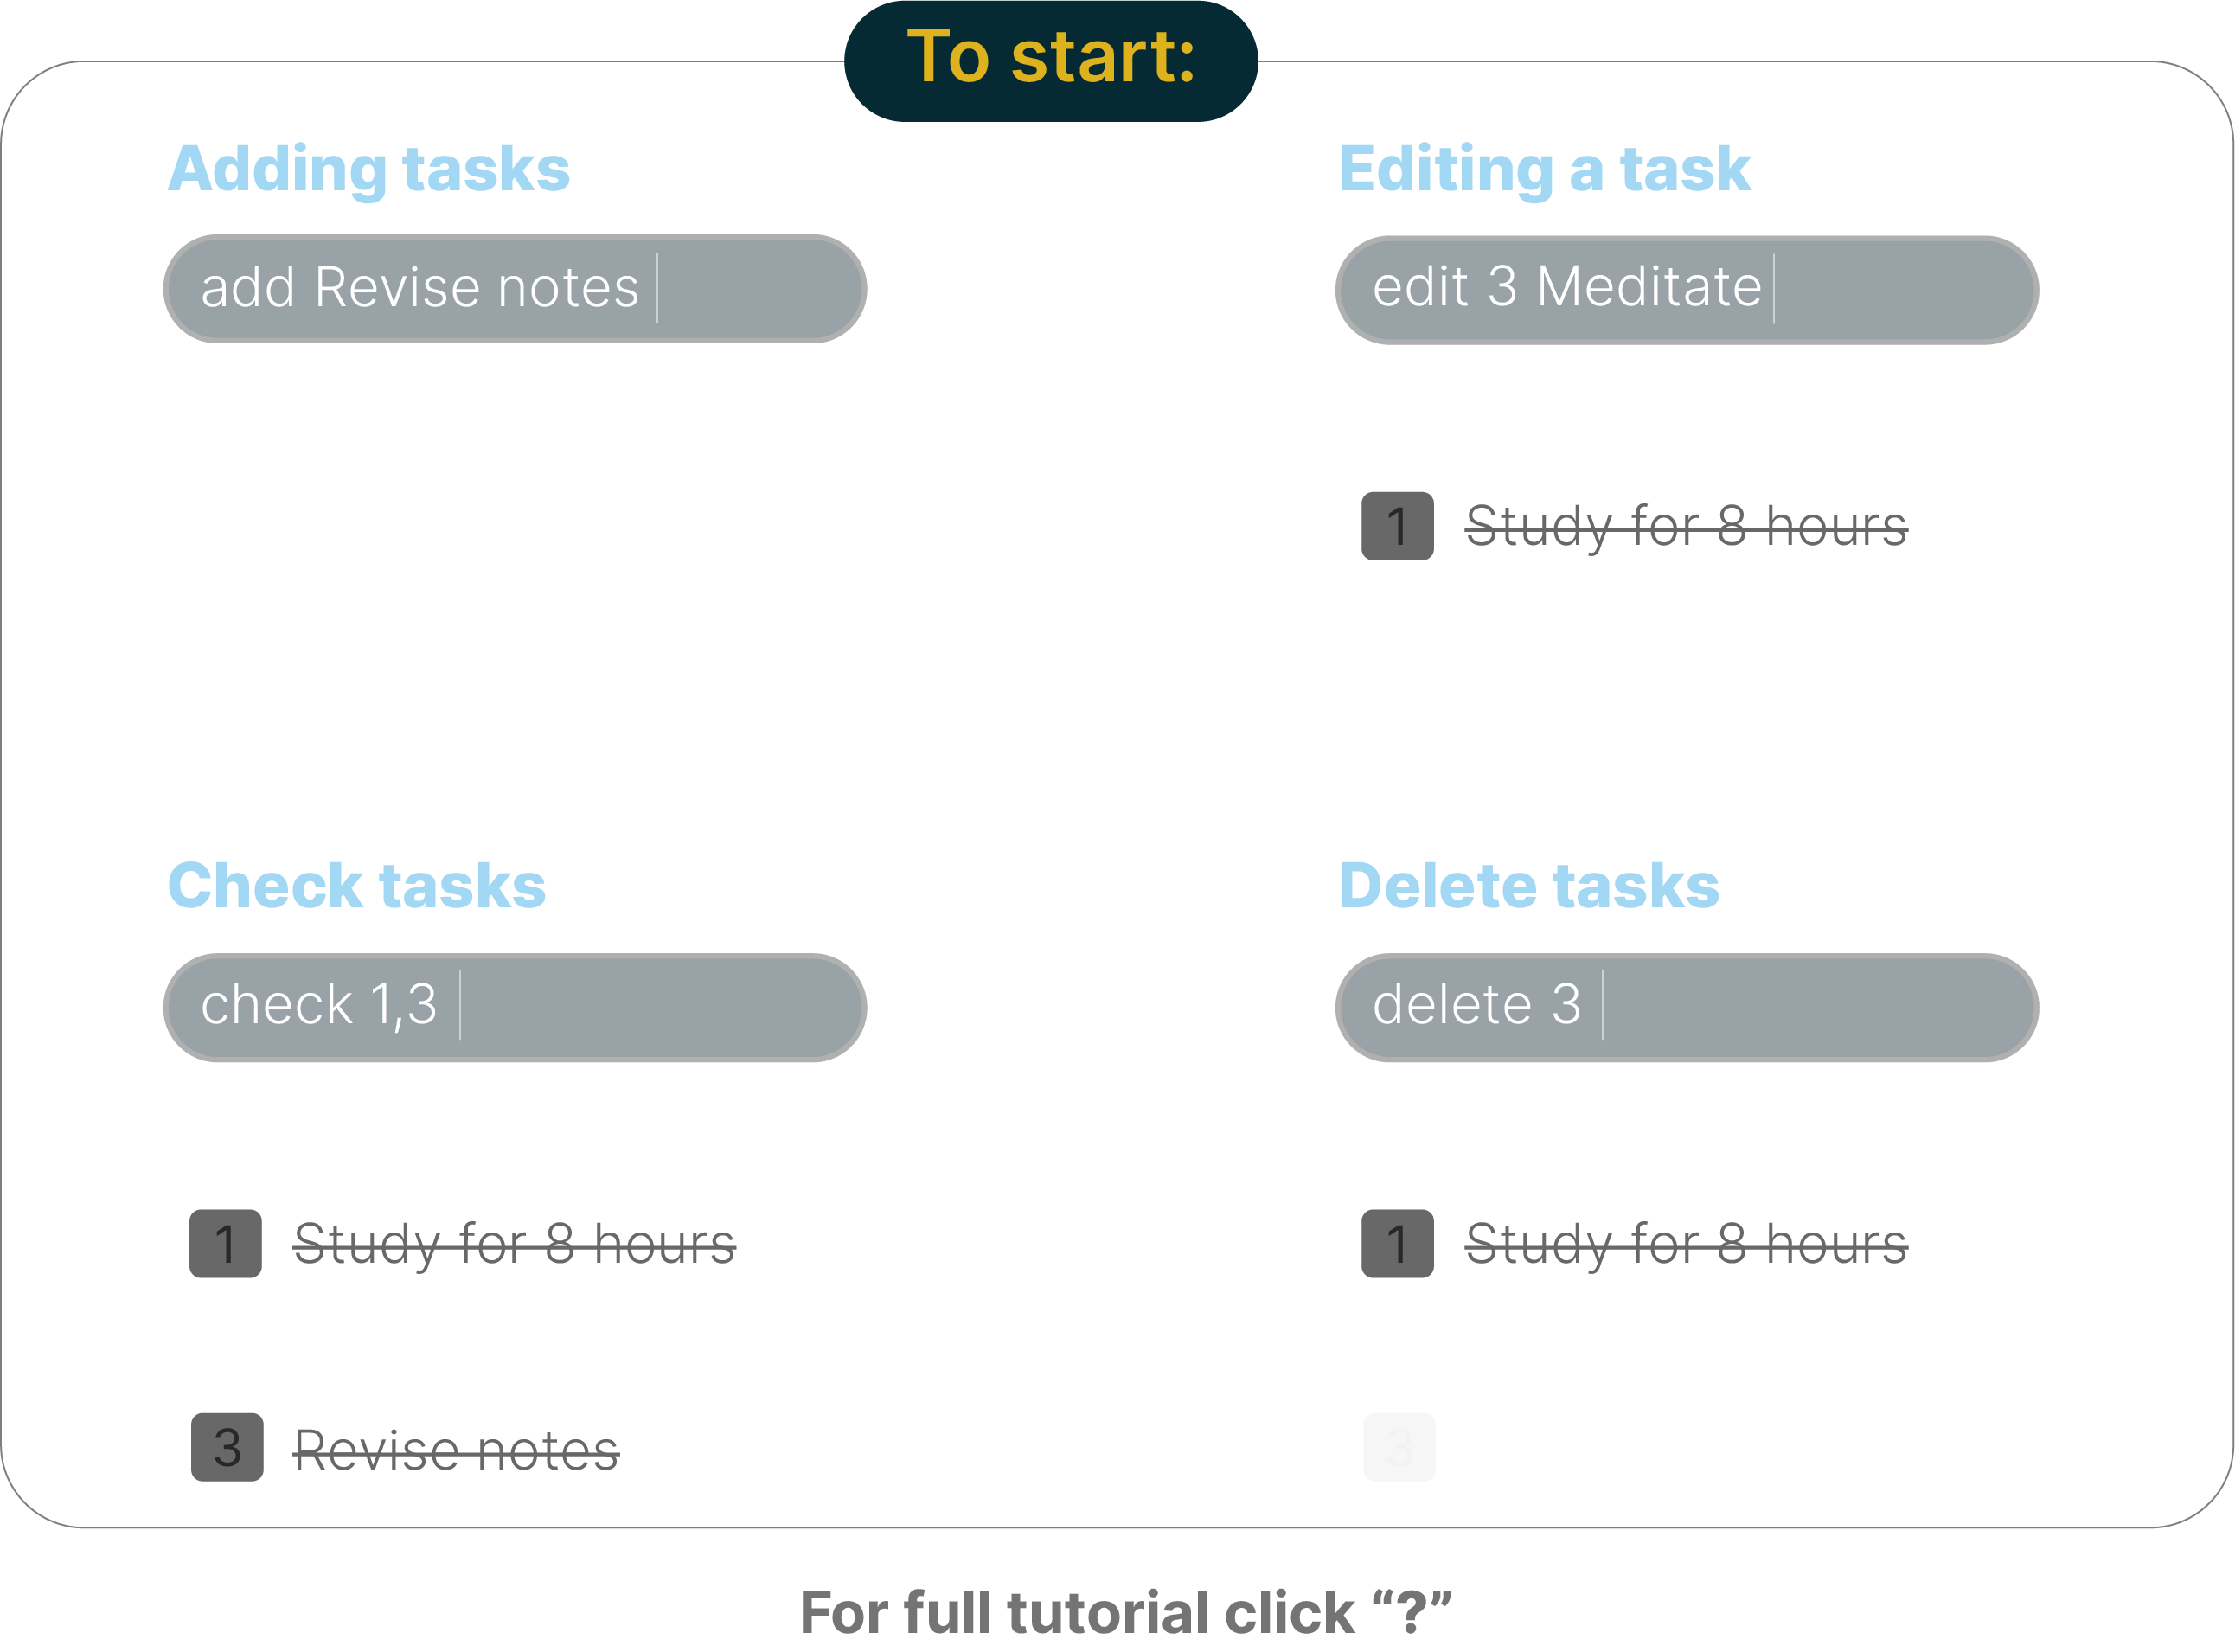
\includegraphics[width=0.25\textwidth, valign=m]{../base/assets/tasklist/help_frame.png}\\
  & \textbf{Default Size} & \texttt{2584x1910}\\
  & \textbf{Default Path} & \texttt{tasklist/help\_frame.png}\\
  \hline
\end{longtable}
\subsection{Mask Assets}
\section{Stats}
\subsection{Colour Properties}
\rowcolors{1}{Tan}{Apricot}
\begin{longtable}{| p{.30\textwidth} p{.45\textwidth} p{.25\textwidth} |}
  \hline
  \rowcolor{gray}
  Property key & Description & In Context \\ \hline \endhead
  \hypertarget{stats-header-colour}{\texttt{header\_colour}} & Colour of the two card headers. &
  \includegraphics[width=.25\textwidth,valign=m]{images/stats/header_colour.png}
  \\
  \hypertarget{stats-stats-subheader-colour}{\texttt{stats\_subheader\_colour}} & Colour of the subheaders in the first column. &
  \includegraphics[width=.25\textwidth,valign=m]{images/stats/stats_subheader_colour.png}
  \\
  \hypertarget{stats-stats-text-colour}{\texttt{stats\_text\_colour}} & Colour of the other text in the first column. &
  \includegraphics[width=.25\textwidth,valign=m]{images/stats/stats_text_colour.png}
  \\
  \hypertarget{stats-col2-date-colour}{\texttt{col2\_date\_colour}} & Colour of the top month and year text in the second column. &
  \includegraphics[width=.25\textwidth,valign=m]{images/stats/col2_date_colour.png}
  \\
  \hypertarget{stats-col2-hours-colour}{\texttt{col2\_hours\_colour}} & Colour of the total hours this month text in the second column. &
  \includegraphics[width=.25\textwidth,valign=m]{images/stats/col2_hours_colour.png}
  \\
  \hypertarget{stats-cal-weekday-colour}{\texttt{cal\_weekday\_colour}} & Colour of the weekdays shown over the calendar. &
  \includegraphics[width=.25\textwidth,valign=m]{images/stats/cal_weekday_colour.png}
  \\
  \hypertarget{stats-cal-number-colour}{\texttt{cal\_number\_colour}} & Colour of the day numbers on the calendar, not including days at the end of streaks. &
  \includegraphics[width=.25\textwidth,valign=m]{images/stats/cal_number_colour.png}
  \\
  \hypertarget{stats-cal-number-end-colour}{\texttt{cal\_number\_end\_colour}} & Colour of the day numbers on the calendar at the end of streaks. &
  \includegraphics[width=.25\textwidth,valign=m]{images/stats/cal_number_end_colour.png}
  \\
  \hypertarget{stats-cal-streak-middle-colour}{\texttt{cal\_streak\_middle\_colour}} & Streak highlight colour shown over middle streak days on the calendar. &
  \includegraphics[width=.25\textwidth,valign=m]{images/stats/cal_streak_middle_colour.png}
  \\
  \hypertarget{stats-cal-streak-end-colour}{\texttt{cal\_streak\_end\_colour}} & Colour of the highlight placed over the end days of streaks.&
  \includegraphics[width=.25\textwidth,valign=m]{images/stats/cal_streak_end_colour.png}
  \\
  \hline
\end{longtable}
\subsection{Spacing Properties}
\subsection{String Properties}
\subsection{Assets}
\groupedRowColors{5}{1}{Tan}{Apricot}
\renewcommand{\arraystretch}{1.2}
\begin{longtable}{| p{.30\textwidth} p{.15\textwidth} p{.55\textwidth}|}
  \hline
  \rowcolor{gray}
  Asset Path Key & \multicolumn{2}{|c|}{Properties} \\ \hline \endhead
  \hypertarget{stats-background}{\texttt{background}} & \multicolumn{2}{p{.70\textwidth+2\tabcolsep}|}{
    Stats card background.
  }\\
  & \textbf{Requirements} & Must have approximately the same dimensions as the default.\\
  & \textbf{Default Asset} & \centering\arraybackslash
\includegraphics[width=0.25\textwidth, valign=m]{../base/assets/stats/background.png}\\
  & \textbf{Default Size} & \texttt{1528x896}\\
  & \textbf{Default Path} & \texttt{stats/background.png}\\[2ex]
  \hline
\end{longtable}
\subsection{Mask Assets}
\section{Profile}
\subsection{Colour Properties}
\rowcolors{1}{Tan}{Apricot}
\begin{longtable}{| p{.30\textwidth} p{.45\textwidth} p{.25\textwidth} |}
  \hline
  \rowcolor{gray}
  Property key & Description & In Context \\ \hline \endhead
  \hypertarget{profile-header-colour-1}{\texttt{header\_colour\_1}} & Colour of the user name in the card header.&
  \includegraphics[width=.25\textwidth,valign=m]{images/profile/header_colour_1.png}
  \\
  \hypertarget{profile-header-colour-2}{\texttt{header\_colour\_2}} & Colour of the discriminator in the card header.&
  \includegraphics[width=.25\textwidth,valign=m]{images/profile/header_colour_2.png}
  \\
  \hypertarget{profile-counter-bg-colour}{\texttt{counter\_bg\_colour}} & Colour of the coin/gem/gift background highlight.&
  \includegraphics[width=.25\textwidth,valign=m]{images/profile/counter_bg_colour.png}
  \\
  \hypertarget{profile-counter-colour}{\texttt{counter\_colour}} & Colour of the coin/gem/gift counter text.&
  \includegraphics[width=.25\textwidth,valign=m]{images/profile/counter_colour.png}
  \\
  \hypertarget{profile-subheader-colour}{\texttt{subheader\_colour}} & Colour of the two card subheaders.&
  \includegraphics[width=.25\textwidth,valign=m]{images/profile/subheader_colour.png}
  \\
  \hypertarget{profile-badge-text-colour}{\texttt{badge\_text\_colour}} & Colour of the text on the profile badges.&
  \includegraphics[width=.25\textwidth,valign=m]{images/profile/badge_text_colour.png}
  \\
  \hypertarget{profile-badge-blob-colour}{\texttt{badge\_blob\_colour}} & Colour of the profile badge backgrounds.&
  \includegraphics[width=.25\textwidth,valign=m]{images/profile/badge_blob_colour.png}
  \\
  \hypertarget{profile-rank-name-colour}{\texttt{rank\_name\_colour}} & Colour of the current rank name. &
  \includegraphics[width=.25\textwidth,valign=m]{images/profile/rank_name_colour.png}
  \\
  \hypertarget{profile-rank-hours-colour}{\texttt{rank\_hours\_colour}} & Colour of the required hours shown for the current rank. &
  \includegraphics[width=.25\textwidth,valign=m]{images/profile/rank_hours_colour.png}
  \\
  \hypertarget{profile-bar-full-colour}{\texttt{bar\_full\_colour}} & Colour of the filled progress bar. (May be overridden with a background asset for e.g. gradients.)&
  \includegraphics[width=.25\textwidth,valign=m]{images/profile/bar_full_colour.png}
  \\
  \hypertarget{profile-bar-empty-colour}{\texttt{bar\_empty\_colour}} & Colour of the progress bar background, or the empty progress bar. (May be overridden with a background asset for e.g. gradients.)&
  \includegraphics[width=.25\textwidth,valign=m]{images/profile/bar_empty_colour.png}
  \\
  \hypertarget{profile-next-rank-colour}{\texttt{next\_rank\_colour}} & Colour of the next rank text displayed under the progress bar.&
  \includegraphics[width=.25\textwidth,valign=m]{images/profile/next_rank_colour.png}
  \\
  \hline
\end{longtable}
\subsection{Spacing Properties}
\subsection{String Properties}
\subsection{Assets}
\groupedRowColors{5}{1}{Tan}{Apricot}
\renewcommand{\arraystretch}{1.2}
\begin{longtable}{| p{.30\textwidth} p{.15\textwidth} p{.55\textwidth}|}
  \hline
  \rowcolor{gray}
  Asset Path Key & \multicolumn{2}{|c|}{Properties} \\ \hline \endhead
  \hypertarget{profile-background}{\texttt{background}} & \multicolumn{2}{p{.70\textwidth+2\tabcolsep}|}{
    Profile card background.
  }\\
  & \textbf{Requirements} & Must have approximately the same dimensions as the default.\\
  & \textbf{Default Asset} & \centering\arraybackslash
\includegraphics[width=0.25\textwidth, valign=m]{../base/assets/profile/background.png}\\
  & \textbf{Default Size} & \texttt{1537x709}\\
  & \textbf{Default Path} & \texttt{profile/background.png}\\[2ex]
  \hypertarget{profile-avatar-outline}{\texttt{avatar\_outline}} & \multicolumn{2}{p{.70\textwidth+2\tabcolsep}|}{
    Avatar border.
    This asset may also be affected or specified by user properties.
    Note the specific size requirements.

    The avatar is first masked (using \texttt{avatar\_mask}), then placed \emph{behind} on this asset image, with matching centres.
    Transparency and size choices should take into account the mask.

    If the mask is significantly larger than the default, the relevant spacing properties should also be modified to preserve the aesthetics of the first profile card column.
  }\\
  & \textbf{Requirements} & Inner dimensions must accommodate a $256\times256$ masked avatar.\newline Asset dimensions should be as close as possible to the default dimensions.\\
  & \textbf{Default Asset} & \centering\arraybackslash
\includegraphics[width=0.1\textwidth, valign=m]{../base/assets/profile/avatar_outline.png}\\
  & \textbf{Default Size} & \texttt{264x264}\\
  & \textbf{Default Path} & \texttt{profile/avatar\_outline.png}\\[2ex]
  \hypertarget{profile-coin-icon}{\texttt{coin\_icon}} & \multicolumn{2}{p{.70\textwidth+2\tabcolsep}|}{
    Icon for the coin counter.

    This image is centred in the \texttt{counter\_background} blob, and should be padded, trimmed, or aligned so the asset centre matches the visual centre.
  }\\
  & \textbf{Requirements} & Must be smaller than the counter background, and have aligned image centre.\\
  & \textbf{Default Asset} & \centering\arraybackslash
\includegraphics[width=0.1\textwidth, valign=m]{../base/assets/icons/coin.png}\\
  & \textbf{Default Size} & \texttt{89x90}\\
  & \textbf{Default Path} & \texttt{icons/coin.png}\\[2ex]
  \hypertarget{profile-gem-icon}{\texttt{gem\_icon}} & \multicolumn{2}{p{.70\textwidth+2\tabcolsep}|}{
    Icon for the gem counter.

    This image is centred in the \texttt{counter\_background} blob, and should be padded, trimmed, or aligned so the asset centre matches the visual centre.
  }\\
  & \textbf{Requirements} & Must be smaller than the counter background, and have aligned image centre.\\
  & \textbf{Default Asset} & \centering\arraybackslash
\includegraphics[width=0.1\textwidth, valign=m]{../base/assets/icons/gem.png}\\
  & \textbf{Default Size} & \texttt{39x38}\\
  & \textbf{Default Path} & \texttt{icons/gem.png}\\[2ex]
  \hypertarget{profile-gift-icon}{\texttt{gift\_icon}} & \multicolumn{2}{p{.70\textwidth+2\tabcolsep}|}{
    Icon for the gift counter.

    This image is centred in the \texttt{counter\_background} blob, and should be padded, trimmed, or aligned so the asset centre matches the visual centre.
  }\\
  & \textbf{Requirements} & Must be smaller than the counter background, and have aligned image centre.\\
  & \textbf{Default Asset} & \centering\arraybackslash
\includegraphics[width=0.1\textwidth, valign=m]{../base/assets/icons/gift.png}\\
  & \textbf{Default Size} & \texttt{75x75}\\
  & \textbf{Default Path} & \texttt{icons/gift.png}\\[2ex]
  \hypertarget{profile-achievements-active}{\texttt{achievements\_active}} & \multicolumn{2}{p{.70\textwidth+2\tabcolsep}|}{
    Relative path (from the asset root) to the folder where the active achievement icons are stored.

    Each icon is pasted in the centre of a $115 \times 96$ (at $150$ DPI) pixel box, which is then placed on a $2\times 8$ grid.
    The dimensions of the icons should take this into consideration, with the visual centres of the icons matching the image centre where possible.
  }\\
  & \textbf{Requirements} & If this is provided, \emph{all} the active achievement icons \emph{must} appear in this folder, and they \emph{must} be labelled from \texttt{1.png} to \texttt{8.png} in the (right to left, top to bottom) order they should appear on the card.\newline For optimal appearance, each icon should have matching visual and actual centre, and should not have dimensions exceeding $115 \times 96$.\\
  & \textbf{Default Assets} &
  \centering\arraybackslash
  \begin{tabular}{cccc}
    
\includegraphics[width=0.1\textwidth, valign=m]{../base/assets/profile/achievements_active/1.png} &
    
\includegraphics[width=0.1\textwidth, valign=m]{../base/assets/profile/achievements_active/2.png} & 
    
\includegraphics[width=0.1\textwidth, valign=m]{../base/assets/profile/achievements_active/3.png} & 
    
\includegraphics[width=0.1\textwidth, valign=m]{../base/assets/profile/achievements_active/4.png} \\
    \includegraphics[width=0.1\textwidth, valign=m]{../base/assets/profile/achievements_active/5.png} &
    \includegraphics[width=0.1\textwidth, valign=m]{../base/assets/profile/achievements_active/6.png} & 
    \includegraphics[width=0.1\textwidth, valign=m]{../base/assets/profile/achievements_active/7.png} & 
    \includegraphics[width=0.1\textwidth, valign=m]{../base/assets/profile/achievements_active/8.png}
  \end{tabular} \\
  & \textbf{Default Size} &
  \centering\arraybackslash
 \(\begin{matrix}75 \times 77 & 63 \times 96 & 115 \times 74 & 86 \times 83\\ 98 \times 77 & 85 \times 83 & 93 \times 78 & 91 \times 83\end{matrix}\)\\
  & \textbf{Default Path} & \texttt{profile/achievements\_active/}\\[2ex]
  \hypertarget{profile-achievements-inactive}{\texttt{achievements\_inactive}} & \multicolumn{2}{p{.70\textwidth+2\tabcolsep}|}{
    Relative path (from the asset root) to the folder where the inactive achievement icons are stored.

    Each icon is pasted in the centre of a $115 \times 96$ (at $150$ DPI) pixel box, which is then placed on a $2\times 8$ grid.
    The dimensions of the icons should take this into consideration, with the visual centres of the icons matching the image centre where possible.
  }\\
  & \textbf{Requirements} & If this is provided, \emph{all} the inactive achievement icons \emph{must} appear in this folder, and they \emph{must} be labelled from \texttt{1.png} to \texttt{8.png} in the (right to left, top to bottom) order they should appear on the card.\newline For optimal appearance, each icon should have matching visual and actual centre, and should not have dimensions exceeding $115 \times 96$.\\
  & \textbf{Default Assets} &
  \centering\arraybackslash
  \begin{tabular}{cccc}
    \includegraphics[width=0.1\textwidth, valign=m]{../base/assets/profile/achievements_inactive/1.png} &
    \includegraphics[width=0.1\textwidth, valign=m]{../base/assets/profile/achievements_inactive/2.png} & 
    \includegraphics[width=0.1\textwidth, valign=m]{../base/assets/profile/achievements_inactive/3.png} & 
    \includegraphics[width=0.1\textwidth, valign=m]{../base/assets/profile/achievements_inactive/4.png} \\
    \includegraphics[width=0.1\textwidth, valign=m]{../base/assets/profile/achievements_inactive/5.png} &
    \includegraphics[width=0.1\textwidth, valign=m]{../base/assets/profile/achievements_inactive/6.png} & 
    \includegraphics[width=0.1\textwidth, valign=m]{../base/assets/profile/achievements_inactive/7.png} & 
    \includegraphics[width=0.1\textwidth, valign=m]{../base/assets/profile/achievements_inactive/8.png}
  \end{tabular} \\
  & \textbf{Default Size} &
  \centering\arraybackslash
 \(\begin{matrix}75 \times 77 & 63 \times 96 & 115 \times 74 & 86 \times 83\\ 98 \times 77 & 85 \times 83 & 93 \times 78 & 91 \times 83\end{matrix}\)\\
  & \textbf{Default Path} & \texttt{profile/achievements\_inactive/}\\[2ex]
  \hline
\end{longtable}
To add: optional \texttt{bar\_full} and \texttt{bar\_empty} assets. Need to create samples for these from mask and colour.
\subsection{Mask Assets}
\section{Weekly Stats}
\textbf{Note:} The weekly stats card is special in that it was initially exported at $72$ pixels per inch instead of $150$ pixels per inch that the rest of the cards use. All sizes and assets for this card must therefore also be in this print resolution, making the weekly card unable to share any assets with other cards. Not that this does not apply to spacing properties, since they are always given in $72$ PPI, and are manually scaled for cards at higher resolutions. Since the weekly stats card can essentially only share the background asset, this should normally not be an issue, but be aware that this difference may be removed in a future update.
\subsection{Colour Properties}
\rowcolors{1}{Tan}{Apricot}
\begin{longtable}{| p{.30\textwidth} p{.45\textwidth} p{.25\textwidth} |}
  \hline
  \rowcolor{gray}
  Property key & Description & In Context \\ \hline \endhead
  \hypertarget{weekly-title-colour}{\texttt{title\_colour}} & Colour of the weekly stats card title. &
  \includegraphics[width=.25\textwidth,valign=m]{images/weekly/title_colour.png}
  \\
  \hypertarget{weekly-top-hours-colour}{\texttt{top\_hours\_colour}} & Colour of the hour axis label text on the top graph. &
  \includegraphics[width=.25\textwidth,valign=m]{images/weekly/top_hours_colour.png}
  \\
  \hypertarget{weekly-top-hours-bg-colour}{\texttt{top\_hours\_bg\_colour}} & Colour of the hour axis label background on the top graph. &
  \includegraphics[width=.25\textwidth,valign=m]{images/weekly/top_hours_bg_colour.png}
  \\
  \hypertarget{weekly-top-line-colour}{\texttt{top\_line\_colour}} & Colour of the horizontal lines on the top graph. &
  \includegraphics[width=.25\textwidth,valign=m]{images/weekly/top_line_colour.png}
  \\
  \hypertarget{weekly-top-weekday-colour}{\texttt{top\_weekday\_colour}} & Colour of the weekdays in the top graph weekday axis labels. &
  \includegraphics[width=.25\textwidth,valign=m]{images/weekly/top_weekday_colour.png}
  \\
  \hypertarget{weekly-top-date-colour}{\texttt{top\_date\_colour}} & Colour of the dates in the top graph weekday axis labels. &
  \includegraphics[width=.25\textwidth,valign=m]{images/weekly/top_date_colour.png}
  \\
  \hypertarget{weekly-top-this-colour}{\texttt{top\_this\_colour}} & Fill colour representing the current week's hours on the top graph, and the bottom legend. &
  \includegraphics[width=.25\textwidth,valign=m]{images/weekly/top_this_colour.png}
  \\
  \hypertarget{weekly-top-last-colour}{\texttt{top\_last\_colour}} & Fill colour representing the last week's hours on the top graph, and the bottom legend. Usually transparent. &
  \includegraphics[width=.25\textwidth,valign=m]{images/weekly/top_last_colour.png}
  \\
  \hypertarget{weekly-btm-weekly-background-colour}{\texttt{btm\_weekly\_background\_colour}} & Colour of the weekday axis background on the bottom graph. &
  \includegraphics[width=.25\textwidth,valign=m]{images/weekly/btm_weekly_background_colour.png}
  \\
  \hypertarget{weekly-btm-bar-horiz-colour}{\texttt{btm\_bar\_horiz\_colour}} & Colour of the horizontal background bars representing days on the bottom graph.&
  \includegraphics[width=.25\textwidth,valign=m]{images/weekly/btm_bar_horiz_colour.png}
  \\
  \hypertarget{weekly-btm-bar-vert-colour}{\texttt{btm\_bar\_vert\_colour}} & Colour of the vertical background bars representing hours on the bottom graph. &
  \includegraphics[width=.25\textwidth,valign=m]{images/weekly/btm_bar_vert_colour.png}
  \\
  \hypertarget{weekly-btm-weekday-colour}{\texttt{btm\_weekday\_colour}} & Colour of the weekday axis text on the bottom graph. &
  \includegraphics[width=.25\textwidth,valign=m]{images/weekly/btm_weekday_colour.png}
  \\
  \hypertarget{weekly-btm-day-colour}{\texttt{btm\_day\_colour}} & Colour of the hour axis text on the bottom graph. &
  \includegraphics[width=.25\textwidth,valign=m]{images/weekly/btm_day_colour.png}
  \\
  \hypertarget{weekly-btm-this-colour}{\texttt{btm\_this\_colour}} & Colour representing the current week's hours on the bottom graph. &
  \includegraphics[width=.25\textwidth,valign=m]{images/weekly/btm_this_colour.png}
  \\
  \hypertarget{weekly-btm-last-colour}{\texttt{btm\_last\_colour}} & Colour representing the last week's hours on the bottom graph. Usually transparent.&
  \includegraphics[width=.25\textwidth,valign=m]{images/weekly/btm_last_colour.png}
  \\
  \hypertarget{weekly-this-week-colour}{\texttt{this\_week\_colour}} & Colour of the legend text for this week. &
  \includegraphics[width=.25\textwidth,valign=m]{images/weekly/this_week_colour.png}
  \\
  \hypertarget{weekly-last-week-colour}{\texttt{last\_week\_colour}} & Colour of the legend text for last week. &
  \includegraphics[width=.25\textwidth,valign=m]{images/weekly/last_week_colour.png}
  \\
  \hypertarget{weekly-footer-colour}{\texttt{footer\_colour}} & Colour of the footer text. &
  \includegraphics[width=.25\textwidth,valign=m]{images/weekly/footer_colour.png}
  \\
  \hline
\end{longtable}
\subsection{Spacing Properties}
\subsection{String Properties}
\subsection{Assets}
\groupedRowColors{5}{1}{Tan}{Apricot}
\renewcommand{\arraystretch}{1.2}
\begin{longtable}{| p{.30\textwidth} p{.15\textwidth} p{.55\textwidth}|}
  \hline
  \rowcolor{gray}
  Asset Path Key & \multicolumn{2}{|c|}{Properties} \\ \hline \endhead
  \hypertarget{weekly-background}{\texttt{background}} & \multicolumn{2}{p{.70\textwidth+2\tabcolsep}|}{
    Weekly stats card background.
  }\\
  & \textbf{Requirements} & Must have approximately the same dimensions as the default.\\
  & \textbf{Default Asset} & \centering\arraybackslash\includegraphics[width=0.25\textwidth, valign=m]{../base/assets/weekly/background.png}\\
  & \textbf{Default Size} & \texttt{1334x1458} \textbf{(72 PPI)}\\
  & \textbf{Default Path} & \texttt{weekly/background.png}\\[2ex]
  \hypertarget{weekly-btm-emoji-path}{\texttt{btm\_emoji\_path}} & \multicolumn{2}{p{.70\textwidth+2\tabcolsep}|}{
    Relative path (from the asset root) to the folder where the five bottom graph daily rating emojis are stored.

    These emojis are placed on the card without modification next to the horizontal day bar on the bottom graph to indicate relative performance
    (by total hour count relative to average) in that day.
  }\\
  & \textbf{Requirements} & If the path property is modified, all five of the rating emojis \emph{must} be appear in the folder,
  or in the same relative location in some parent skin. If the path property is \emph{not} modified, the emojis may be individually
  overridden by supplying a file of the correct name in the correct location, similarly to regular assets.\newline
  Supplied emojis \emph{must} have the same names as the default emojis.\newline
  Supplied emojis \emph{should} have approximately the same size as the default emojis, since they are not resized before being placed on the card.
  \\
  & \textbf{Default Assets} &
    \centering\arraybackslash
    \begin{tabular}{cc}
      \texttt{shocked.png}     & \includegraphics[width=0.1\textwidth, valign=m]{../base/assets/weekly/emojis/shocked.png} \\
      \texttt{sad.png}         & \includegraphics[width=0.1\textwidth, valign=m]{../base/assets/weekly/emojis/sad.png} \\
      \texttt{neutral.png}     & \includegraphics[width=0.1\textwidth, valign=m]{../base/assets/weekly/emojis/neutral.png} \\
      \texttt{happy.png}       & \includegraphics[width=0.1\textwidth, valign=m]{../base/assets/weekly/emojis/happy.png} \\
      \texttt{very\_happy.png} & \includegraphics[width=0.1\textwidth, valign=m]{../base/assets/weekly/emojis/very\_happy.png}
    \end{tabular}
  \\
  & \textbf{Default Sizes} &
  \(
    \begin{matrix}
      34\times 34 & 34 \times 35 & 34 \times 35 & 34 \times 35 & 34 \times 34
    \end{matrix}
  \)
  \\
  & \textbf{Default Path} & \texttt{weekly/emojis}\\[2ex]
  \hline
\end{longtable}
To add: optional \texttt{top\_hours\_bg}, \texttt{top\_this\_bar\_full}, \texttt{top\_last\_bar\_full}, \texttt{btm\_this\_end}, \texttt{btm\_last\_end}, \texttt{this\_week\_image}, \texttt{last\_week\_image} blob assets. Need to create samples for these from mask and colour.
\subsection{Mask Assets}
\section{Monthly Stats}
\subsection{Colour Properties}
\rowcolors{1}{Tan}{Apricot}
\begin{longtable}{| p{.30\textwidth} p{.45\textwidth} p{.25\textwidth} |}
  \hline
  \rowcolor{gray}
  Property key & Description & In Context \\ \hline \endhead
  \hypertarget{monthly-title-colour}{\texttt{title\_colour}} & Colour of the card title text.&
  \includegraphics[width=.25\textwidth,valign=m]{images/monthly/title_colour.png}
  \\
  \hypertarget{monthly-top-hours-colour}{\texttt{top\_hours\_colour}} & Colour of the hour axis label text on the top graph. &
  \includegraphics[width=.25\textwidth,valign=m]{images/monthly/top_hours_colour.png}
  \\
  \hypertarget{monthly-top-hours-bg-colour}{\texttt{top\_hours\_bg\_colour}} & Colour of the hour axis label background on the top graph. &
  \includegraphics[width=.25\textwidth,valign=m]{images/monthly/top_hours_bg_colour.png}
  \\
  \hypertarget{monthly-top-line-colour}{\texttt{top\_line\_colour}} & Colour of the horizontal lines on the top graph. &
  \includegraphics[width=.25\textwidth,valign=m]{images/monthly/top_line_colour.png}
  \\
  \hypertarget{monthly-top-date-colour}{\texttt{top\_date\_colour}} & Colour of the day axis label text on the top graph. &
  \includegraphics[width=.25\textwidth,valign=m]{images/monthly/top_date_colour.png}
  \\
  \hypertarget{monthly-top-this-colour}{\texttt{top\_this\_colour}} & Fill colour representing this month's hours on the top graph, and the legend.&
  \includegraphics[width=.25\textwidth,valign=m]{images/monthly/top_this_colour.png}
  \\
  \hypertarget{monthly-top-last-colour}{\texttt{top\_last\_colour}} & Fill colour representing last month's hours on the top graph, and the legend. Often transparent.&
  \includegraphics[width=.25\textwidth,valign=m]{images/monthly/top_last_colour.png}
  \\
  \hypertarget{monthly-top-this-hours-colour}{\texttt{top\_this\_hours\_colour}} & Text colour for the number of hours studied each day of this month, printed above each bar on the top graph. &
  \includegraphics[width=.25\textwidth,valign=m]{images/monthly/top_this_hours_colour.png}
  \\
  \hypertarget{monthly-top-last-hours-colour}{\texttt{top\_last\_hours\_colour}} & Text colour for the number of hours studied each day of last month, printed above each bar on the top graph. &
  \includegraphics[width=.25\textwidth,valign=m]{images/monthly/top_last_hours_colour.png}
  \\
  \hypertarget{monthly-this-month-colour}{\texttt{this\_month\_colour}} & This month's text colour in the graph legend. &
  \includegraphics[width=.25\textwidth,valign=m]{images/monthly/this_month_colour.png}
  \\
  \hypertarget{monthly-last-month-colour}{\texttt{last\_month\_colour}} & Last month's text colour in the graph legend. &
  \includegraphics[width=.25\textwidth,valign=m]{images/monthly/last_month_colour.png}
  \\
  \hypertarget{monthly-weekday-background-colour}{\texttt{weekday\_background\_colour}} & Colour of the weekday axis label background on the bottom heatmap.&
  \includegraphics[width=.25\textwidth,valign=m]{images/monthly/weekday_background_colour.png}
  \\
  \hypertarget{monthly-weekday-colour}{\texttt{weekday\_colour}} & Colour of the weekday axis label text on the bottom heatmap.&
  \includegraphics[width=.25\textwidth,valign=m]{images/monthly/weekday_colour.png}
  \\
  \hypertarget{monthly-month-background-colour}{\texttt{month\_background\_colour}} & Colour of the month axis label background on the bottom heatmap. &
  \includegraphics[width=.25\textwidth,valign=m]{images/monthly/month_background_colour.png}
  \\
  \hypertarget{monthly-month-colour}{\texttt{month\_colour}} & Colour of the month axis label text on the bottom heatmap. &
  \includegraphics[width=.25\textwidth,valign=m]{images/monthly/month_colour.png}
  \\
  \hypertarget{monthly-heatmap-empty-colour}{\texttt{heatmap\_empty\_colour}} & Colour used in the heatmap when no study occurred on that day. &
  \includegraphics[width=.25\textwidth,valign=m]{images/monthly/heatmap_empty_colour.png}
  \\
  \hypertarget{monthly-stats-key-colour}{\texttt{stats\_key\_colour}} & Text colour of the summary statistic names printed below the heatmap. &
  \includegraphics[width=.25\textwidth,valign=m]{images/monthly/stats_key_colour.png}
  \\
  \hypertarget{monthly-stats-value-colour}{\texttt{stats\_value\_colour}} & Text colour of the summary statistic values printed below the heatmap. &
  \includegraphics[width=.25\textwidth,valign=m]{images/monthly/stats_value_colour.png}
  \\
  \hypertarget{monthly-footer-colour}{\texttt{footer\_colour}} & Text colour of the card footer. &
  \includegraphics[width=.25\textwidth,valign=m]{images/monthly/footer_colour.png}
  \\
  \hypertarget{monthly-heatmap-colours}{\texttt{heatmap\_colours}} & \emph{List} of colours used in the heatmap to represent relative study amounts for each day. This list may be of any positive length.\newline To choose a colour for a given day, the user's average all-time hours/day is calculated, then the number of hours for that day is placed on a scale from $0$ (non-inclusive) to twice their average (any excess time over twice their average is ignored). A colour is then chosen from the same position on the list of colours as the day's hours on the hour scale.&
  \includegraphics[width=.25\textwidth,valign=t]{images/monthly/heatmap_colours.png}
  \\
\end{longtable}
\subsection{Spacing Properties}
\subsection{String Properties}
\subsection{Assets}
\groupedRowColors{5}{1}{Tan}{Apricot}
\renewcommand{\arraystretch}{1.2}
\begin{longtable}{| p{.30\textwidth} p{.15\textwidth} p{.55\textwidth}|}
  \hline
  \rowcolor{gray}
  Asset Path Key & \multicolumn{2}{|c|}{Properties} \\ \hline \endhead
  \hypertarget{monthly-background}{\texttt{background}} & \multicolumn{2}{p{.70\textwidth+2\tabcolsep}|}{
    Monthly stats card background.
  }\\
  & \textbf{Requirements} & Must have approximately the same dimensions as the default.\\
  & \textbf{Default Asset} & \centering\arraybackslash\includegraphics[width=0.25\textwidth, valign=m]{../base/assets/monthly/background.png}\\
  & \textbf{Default Size} & \texttt{2779x3036}\\
  & \textbf{Default Path} & \texttt{monthly/background.png}\\[2ex]
  \hypertarget{monthly-bottom-frame}{\texttt{bottom\_frame}} & \multicolumn{2}{p{.70\textwidth+2\tabcolsep}|}{
    Thin bottom frame surrounding the heatmap.
  }\\
  & \textbf{Requirements} & Must have approximately the same dimensions as the default.\\
  & \textbf{Default Asset} & \centering\arraybackslash\includegraphics[width=0.25\textwidth, valign=m]{../base/assets/monthly/bottom_frame.png}\\
  & \textbf{Default Size} & \texttt{2645x1041}\\
  & \textbf{Default Path} & \texttt{monthly/bottom\_frame.png}\\[2ex]
  \hline
\end{longtable}
To add: Lots of optional blob assets and masks supporting custom blob and bar backgrounds.
\subsection{Mask Assets}
\section{Weekly Goals}
\subsection{Colour Properties}
\rowcolors{1}{Tan}{Apricot}
\begin{longtable}{| p{.30\textwidth} p{.45\textwidth} p{.25\textwidth} |}
  \hline
  \rowcolor{gray}
  Property key & Description & In Context \\ \hline \endhead
  \hypertarget{weeklygoals-title-colour}{\texttt{title\_colour}} & Text colour of the card title. &
  \includegraphics[width=.25\textwidth,valign=m]{images/weeklygoals/title_colour.png}
  \\
  \hypertarget{weeklygoals-mini-profile-name-colour}{\texttt{mini\_profile\_name\_colour}} & Colour of the user name in the mini-profile. &
  \includegraphics[width=.25\textwidth,valign=m]{images/weeklygoals/mini_profile_name_colour.png}
  \\
  \hypertarget{weeklygoals-mini-profile-discrim-colour}{\texttt{mini\_profile\_discrim\_colour}} & Colour of the user discriminator in the mini-profile. &
  \includegraphics[width=.25\textwidth,valign=m]{images/weeklygoals/mini_profile_discrim_colour.png}
  \\
  \hypertarget{weeklygoals-mini-profile-badge-colour}{\texttt{mini\_profile\_badge\_colour}} & Colour of the mini-profile badge backgrounds. &
  \includegraphics[width=.25\textwidth,valign=m]{images/weeklygoals/mini_profile_badge_colour.png}
  \\
  \hypertarget{weeklygoals-mini-profile-badge-text-colour}{\texttt{mini\_profile\_badge\_text\_colour}} & Colour of the mini-profile badge text. &
  \includegraphics[width=.25\textwidth,valign=m]{images/weeklygoals/mini_profile_badge_text_colour.png}
  \\
  \hypertarget{weeklygoals-progress-bg-colour}{\texttt{progress\_bg\_colour}} & Background/unfilled colour of the circular progress bars. &
  \includegraphics[width=.25\textwidth,valign=m]{images/weeklygoals/progress_bg_colour.png}
  \\
  \hypertarget{weeklygoals-progress-colour}{\texttt{progress\_colour}} & Foreground/filled colour of the circular progress bars. &
  \includegraphics[width=.25\textwidth,valign=m]{images/weeklygoals/progress_colour.png}
  \\
  \hypertarget{weeklygoals-task-count-colour}{\texttt{task\_count\_colour}} & Colour of the number of tasks complete. &
  \includegraphics[width=.25\textwidth,valign=m]{images/weeklygoals/task_count_colour.png}
  \\
  \hypertarget{weeklygoals-task-done-colour}{\texttt{task\_done\_colour}} & Colour of the "tasks\_done" text. &
  \includegraphics[width=.25\textwidth,valign=m]{images/weeklygoals/task_done_colour.png}
  \\
  \hypertarget{weeklygoals-task-goal-colour}{\texttt{task\_goal\_colour}} & Colour of the task "Goal" text. &
  \includegraphics[width=.25\textwidth,valign=m]{images/weeklygoals/task_goal_colour.png}
  \\
  \hypertarget{weeklygoals-task-goal-number-colour}{\texttt{task\_goal\_number\_colour}} & Text colour for the numerical task goal. &
  \includegraphics[width=.25\textwidth,valign=m]{images/weeklygoals/task_goal_number_colour.png}
  \\
  \hypertarget{weeklygoals-studied-text-colour}{\texttt{studied\_text\_colour}} & Colour of the default text on the "Studied" progress bar. &
  \includegraphics[width=.25\textwidth,valign=m]{images/weeklygoals/studied_text_colour.png}
  \\
  \hypertarget{weeklygoals-studied-hour-colour}{\texttt{studied\_hour\_colour}} & Colour of the progress text on the "Studied" progress bar. &
  \includegraphics[width=.25\textwidth,valign=m]{images/weeklygoals/studied_hour_colour.png}
  \\
  \hypertarget{weeklygoals-attendance-rate-colour}{\texttt{attendance\_rate\_colour}} & Colour of the attendance rate on the "attendance" bar. &
  \includegraphics[width=.25\textwidth,valign=m]{images/weeklygoals/attendance_rate_colour.png}
  \\
  \hypertarget{weeklygoals-attendance-colour}{\texttt{attendance\_colour}} & Colour of the text on the "attendance" bar. &
  \includegraphics[width=.25\textwidth,valign=m]{images/weeklygoals/attendance_colour.png}
  \\
  \hypertarget{weeklygoals-task-header-colour}{\texttt{task\_header\_colour}} & Colour of the subheader over the textual goals section. &
  \includegraphics[width=.25\textwidth,valign=m]{images/weeklygoals/task_header_colour.png}
  \\
  \hypertarget{weeklygoals-task-done-number-colour}{\texttt{task\_done\_number\_colour}} & Text colour of the number for completed textual goals. &
  \includegraphics[width=.25\textwidth,valign=m]{images/weeklygoals/task_done_number_colour.png}
  \\
  \hypertarget{weeklygoals-task-done-text-colour}{\texttt{task\_done\_text\_colour}} & Text colour of the text for completed textual goals. &
  \includegraphics[width=.25\textwidth,valign=m]{images/weeklygoals/task_done_text_colour.png}
  \\
  \hypertarget{weeklygoals-task-undone-number-colour}{\texttt{task\_undone\_number\_colour}} & Text colour of the number for incomplete textual goals. &
  \includegraphics[width=.25\textwidth,valign=m]{images/weeklygoals/task_undone_number_colour.png}
  \\
  \hypertarget{weeklygoals-task-undone-text-colour}{\texttt{task\_undone\_text\_colour}} & Text colour of the text for incomplete textual goals. &
  \includegraphics[width=.25\textwidth,valign=m]{images/weeklygoals/task_undone_text_colour.png}
  \\
  \hypertarget{weeklygoals-footer-colour}{\texttt{footer\_colour}} & Text colour of the card footer. &
  \includegraphics[width=.25\textwidth,valign=m]{images/weeklygoals/footer_colour.png}
  \\
  \hline
\end{longtable}
\subsection{Spacing Properties}
\subsection{String Properties}
\subsection{Assets}
\groupedRowColors{5}{1}{Tan}{Apricot}
\renewcommand{\arraystretch}{1.2}
\begin{longtable}{| p{.30\textwidth} p{.15\textwidth} p{.55\textwidth}|}
  \hline
  \rowcolor{gray}
  Asset Path Key & \multicolumn{2}{|c|}{Properties} \\ \hline \endhead
  \hypertarget{weeklygoals-background}{\texttt{background}} & \multicolumn{2}{p{.70\textwidth+2\tabcolsep}|}{
    Goal page background.
  }\\
  & \textbf{Requirements} & Must have approximately the same dimensions as the default.\\
  & \textbf{Default Asset} & \centering\arraybackslash\includegraphics[width=0.25\textwidth, valign=m]{../base/assets/goals/background.png}\\
  & \textbf{Default Size} & \texttt{2779x3036}\\
  & \textbf{Default Path} & \texttt{goals/background.png}\\[2ex]
  \hypertarget{weeklygoals-task-frame}{\texttt{task\_frame}} & \multicolumn{2}{p{.70\textwidth+2\tabcolsep}|}{
    Frame displayed around the textual goals on the bottom of the card.
  }\\
  & \textbf{Requirements} & Must have a size compatible with the provided background. Should be similar to the default.\\
  & \textbf{Default Asset} & \centering\arraybackslash\includegraphics[width=0.25\textwidth, valign=m]{../base/assets/goals/task_frame.png}\\
  & \textbf{Default Size} & \texttt{2443x945}\\
  & \textbf{Default Path} & \texttt{goals/task\_frame.png}\\[2ex]
  \hypertarget{weeklygoals-mini-profile-avatar-frame}{\texttt{mini\_profile\_avatar\_frame}} & \multicolumn{2}{p{.70\textwidth+2\tabcolsep}|}{
    Frame displayed around the avatar on the miniature user profile.
  }\\
  & \textbf{Requirements} & Must be as close as possible to the default size. Small variations are allowed, but may require spacing property modification.\\
  & \textbf{Default Asset} & \centering\arraybackslash\includegraphics[width=0.25\textwidth, valign=m]{../base/assets/mini-profile/avatar_frame.png}\\
  & \textbf{Default Size} & \texttt{264x264}\\
  & \textbf{Default Path} & \texttt{mini-profile/avatar\_frame.png}\\[2ex]
  \hypertarget{weeklygoals-task-done-number-bg}{\texttt{task\_done\_number\_bg}} & \multicolumn{2}{p{.70\textwidth+2\tabcolsep}|}{
    Task number background for completed textual goals.
  }\\
  & \textbf{Requirements} & No special requirements.\\
  & \textbf{Default Asset} & \centering\arraybackslash\includegraphics[width=0.1\textwidth, valign=m]{../base/assets/goals/task_done.png}\\
  & \textbf{Default Size} & \texttt{91x87}\\
  & \textbf{Default Path} & \texttt{goals/task\_done.png}\\[2ex]
  \hypertarget{weeklygoals-task-undone-number-bg}{\texttt{task\_undone\_number\_bg}} & \multicolumn{2}{p{.70\textwidth+2\tabcolsep}|}{
    Task number background for incomplete textual goals.
  }\\
  & \textbf{Requirements} & Assumed to have the same size as the \texttt{task\_done\_number\_bg}.\\
  & \textbf{Default Asset} & \centering\arraybackslash\includegraphics[width=0.1\textwidth, valign=m]{../base/assets/goals/task_undone.png}\\
  & \textbf{Default Size} & \texttt{91x87}\\
  & \textbf{Default Path} & \texttt{goals/task\_undone.png}\\
  \hypertarget{weeklygoals-help-frame}{\texttt{help\_frame}} & \multicolumn{2}{p{.70\textwidth+2\tabcolsep}|}{
    The image to place under the miniature profile when there are no tasks to display.
    Intended to assist the user in using the associated user interface.
  }\\
  & \textbf{Requirements} & Must be compatible with the provided background, and should be similar to the default size.\\
  & \textbf{Default Asset} & \centering\arraybackslash\includegraphics[width=0.25\textwidth, valign=m]{../base/assets/weekly/help_frame.png}\\
  & \textbf{Default Size} & \texttt{2443x1808}\\
  & \textbf{Default Path} & \texttt{weekly/help\_frame.png}\\
  \hline
\end{longtable}
\subsection{Mask Assets}
\section{Monthly Goals}
The Monthly Goals card is identical to the Weekly Goals card described above, apart from the default values of the title text, task header text, and help frame asset, given below. We do not repeat the properties to avoid needless redundancy, please refer to the weekly goal properties instead.

In general, skins implementing a goal skin should write the properties into a common (abstract) field (called e.g. \texttt{"\_goals"} as in the example given in the appendix), and then use the \texttt{"parents"} card property to inherit the common properties from the abstract field.
As usual, see the appendix for a worked example.

Note that the weekly and monthly goal cards may still be customised separately, they merely have exactly the same layout and property names,
and thus will usually share most property values in consistent skins.
\subsection{Colour Properties}
\subsection{Spacing Properties}
\subsection{String Properties}
\subsection{Assets}
\groupedRowColors{5}{1}{Tan}{Apricot}
\renewcommand{\arraystretch}{1.2}
\begin{longtable}{| p{.30\textwidth} p{.15\textwidth} p{.55\textwidth}|}
  \hline
  \rowcolor{gray}
  Asset Path Key & \multicolumn{2}{|c|}{Properties} \\ \hline \endhead
  \hypertarget{monthlygoals-help-frame}{\texttt{help\_frame}} & \multicolumn{2}{p{.70\textwidth+2\tabcolsep}|}{
    The image to place under the miniature profile when there are no tasks to display.
    Intended to assist the user in using the associated user interface.
  }\\
  & \textbf{Requirements} & Must be compatible with the provided background, and should be similar to the default size.\\
  & \textbf{Default Asset} & \centering\arraybackslash\includegraphics[width=0.25\textwidth, valign=m]{../base/assets/monthly/help_frame.png}\\
  & \textbf{Default Size} & \texttt{2443x1808}\\
  & \textbf{Default Path} & \texttt{monthly/help\_frame.png}\\
  \hline
\end{longtable}
\subsection{Mask Assets}
\section{Leaderboard}
\rowcolors{1}{Tan}{Apricot}
\begin{longtable}{| p{.30\textwidth} p{.45\textwidth} p{.25\textwidth} |}
  \hline
  \rowcolor{gray}
  Property key & Description & In Context \\ \hline \endhead
  \hypertarget{leaderboard-header-text-colour}{\texttt{header\_text\_colour}} & &
  \includegraphics[width=.25\textwidth,valign=m]{images/leaderboard/header_text_colour.png}
  \\
  \hypertarget{leaderboard-subheader-name-colour}{\texttt{subheader\_name\_colour}} & &
  \includegraphics[width=.25\textwidth,valign=m]{images/leaderboard/subheader_name_colour.png}
  \\
  \hypertarget{leaderboard-subheader-value-colour}{\texttt{subheader\_value\_colour}} & &
  \includegraphics[width=.25\textwidth,valign=m]{images/leaderboard/subheader_value_colour.png}
  \\
  \hypertarget{leaderboard-top-position-colour}{\texttt{top\_position\_colour}} & &
  \includegraphics[width=.25\textwidth,valign=m]{images/leaderboard/top_position_colour.png}
  \\
  \hypertarget{leaderboard-top-name-colour}{\texttt{top\_name\_colour}} & &
  \includegraphics[width=.25\textwidth,valign=m]{images/leaderboard/top_name_colour.png}
  \\
  \hypertarget{leaderboard-top-hours-colour}{\texttt{top\_hours\_colour}} & &
  \includegraphics[width=.25\textwidth,valign=m]{images/leaderboard/top_hours_colour.png}
  \\
  \hypertarget{leaderboard-entry-position-colour}{\texttt{entry\_position\_colour}} & &
  \includegraphics[width=.25\textwidth,valign=m]{images/leaderboard/entry_position_colour.png}
  \\
  \hypertarget{leaderboard-entry-name-colour}{\texttt{entry\_name\_colour}} & &
  \includegraphics[width=.25\textwidth,valign=m]{images/leaderboard/entry_name_colour.png}
  \\
  \hypertarget{leaderboard-entry-hours-colour}{\texttt{entry\_hours\_colour}} & &
  \includegraphics[width=.25\textwidth,valign=m]{images/leaderboard/entry_hours_colour.png}
  \\
  \hypertarget{leaderboard-entry-bg-colour}{\texttt{entry\_bg\_colour}} & &
  \includegraphics[width=.25\textwidth,valign=m]{images/leaderboard/entry_bg_colour.png}
  \\
  \hypertarget{leaderboard-entry-bg-highlight-colour}{\texttt{entry\_bg\_highlight\_colour}} & &
  \includegraphics[width=.25\textwidth,valign=m]{images/leaderboard/entry_bg_highlight_colour.png}
  \\
  \hline
\end{longtable}
\subsection{Colour Properties}
\subsection{Spacing Properties}
\subsection{String Properties}
\subsection{Assets}
\groupedRowColors{5}{1}{Tan}{Apricot}
\renewcommand{\arraystretch}{1.2}
\begin{longtable}{| p{.30\textwidth} p{.15\textwidth} p{.55\textwidth}|}
  \hline
  \rowcolor{gray}
  Asset Path Key & \multicolumn{2}{|c|}{Properties} \\ \hline \endhead
  \hypertarget{leaderboard-first-bg-path}{\texttt{first\_bg\_path}} & \multicolumn{2}{p{.70\textwidth+2\tabcolsep}|}{
    Background of the first leaderboard page, including embedded header.
  }\\
  & \textbf{Requirements} & The dimensions should be approximately the same as the default background. The header may be shorter or taller, but the corresponding spacing property will need to be modified.\\
  & \textbf{Default Asset} & \centering\arraybackslash\includegraphics[width=0.25\textwidth, valign=m]{../base/assets/leaderboard/first_page_background.png}\\
  & \textbf{Default Size} & \texttt{2811x3048}\\
  & \textbf{Default Path} & \texttt{leaderboard/first\_page\_background.png}\\[2ex]
  \hypertarget{leaderboard-other-bg-path}{\texttt{other\_bg\_path}} & \multicolumn{2}{p{.70\textwidth+2\tabcolsep}|}{
    Background of the second and further leaderboard pages, with embedded header.
  }\\
  & \textbf{Requirements} & The dimensions should be approximately the same as the default background. The header may be shorter, taller, or separated more or less from the main card, but the corresponding spacing property will need to be modified.\\
  & \textbf{Default Asset} & \centering\arraybackslash\includegraphics[width=0.25\textwidth, valign=m]{../base/assets/leaderboard/other_page_background.png}\\
  & \textbf{Default Size} & \texttt{2819x3042}\\
  & \textbf{Default Path} & \texttt{leaderboard/other\_page\_background.png}\\[2ex]
  \hypertarget{leaderboard-first-avatar-bg}{\texttt{first\_avatar\_bg}} & \multicolumn{2}{p{.70\textwidth+2\tabcolsep}|}{
    The avatar background of the first-ranking user.
  }\\
  & \textbf{Requirements} & The dimensions of the background must be able to accommodate the $512\times512$ masked avatar. If the dimensions differ too significantly from the default, spacing properties will need to be modified.\\
  & \textbf{Default Asset} & \centering\arraybackslash\includegraphics[width=0.25\textwidth, valign=m]{../base/assets/leaderboard/first_avatar_background.png}\\
  & \textbf{Default Size} & \texttt{565x664}\\
  & \textbf{Default Path} & \texttt{leaderboard/first\_avatar\_background.png}\\[2ex]
  \hypertarget{leaderboard-second-avatar-bg}{\texttt{second\_avatar\_bg}} & \multicolumn{2}{p{.70\textwidth+2\tabcolsep}|}{
    The avatar background of the second-ranking user.
  }\\
  & \textbf{Requirements} & The dimensions of the background must be able to accommodate the $512\times512$ masked avatar. If the dimensions differ too significantly from the default, spacing properties will need to be modified.\\
  & \textbf{Default Asset} & \centering\arraybackslash\includegraphics[width=0.25\textwidth, valign=m]{../base/assets/leaderboard/second_avatar_background.png}\\
  & \textbf{Default Size} & \texttt{451x527}\\
  & \textbf{Default Path} & \texttt{leaderboard/second\_avatar\_background.png}\\[2ex]
  \hypertarget{leaderboard-third-avatar-bg}{\texttt{third\_avatar\_bg}} & \multicolumn{2}{p{.70\textwidth+2\tabcolsep}|}{
    The avatar background of the third-ranking user.
  }\\
  & \textbf{Requirements} & The dimensions of the background must be able to accommodate the $512\times512$ masked avatar. If the dimensions differ too significantly from the default, spacing properties will need to be modified.\\
  & \textbf{Default Asset} & \centering\arraybackslash\includegraphics[width=0.25\textwidth, valign=m]{../base/assets/leaderboard/third_avatar_background.png}\\
  & \textbf{Default Size} & \texttt{451x526}\\
  & \textbf{Default Path} & \texttt{leaderboard/third\_avatar\_background.png}\\[2ex]
  \hline
\end{longtable}
\subsection{Mask Assets}

\appendix
\chapter{Annotated Example: \texttt{Obsidian}}
\section{Directory Structure}
\emph{Click on an asset to jump to its description, default, size, and requirements.}\\
\begin{tikzpicture}%
  \draw[color=black!60!white]
  \FTdir(\FTroot,root,skins){       % root: parent = \FTroot
    \FTfileicon(root,\faFileText,skins.json)
    \FTdir(root,obsidian,obsidian){       % normal dir: (parentID, currentID, label)
      \FTfileicon(obsidian,\faFileText,skin.json)       % file:       (parentID, label)
      \FTdir(obsidian,assets,assets){
        \FTdir(assets,goals,goals){
          \FTimage(goals,\hyperlink{weeklygoals-task-done-number-bg}{task\_done.png})
          \FTimage(goals,\hyperlink{weeklygoals-task-frame}{task\_frame.png})
          \FTimage(goals,\hyperlink{weeklygoals-task-undone-number-bg}{task\_undone.png})
        }
        \FTdir(assets,leaderboard,leaderboard){
          \FTimage(leaderboard,\hyperlink{leaderboard-first-bg-path}{first\_page\_background.png})
          \FTimage(leaderboard,\hyperlink{leaderboard-other-bg-path}{other\_page\_background.png})
        }
        \FTdir(assets,mini-profile,mini-profile){
          \FTimage(mini-profile,\hyperlink{tasklist-mini-profile-avatar-frame}{avatar\_frame.png})
        }
        \FTdir(assets,shared,shared){
          \FTimage(shared,\hyperlink{weeklygoals-background}{first\_page\_background.png})
          \FTimage(shared,\hyperlink{monthly-background}{second\_page\_background.png})
        }
        \FTdir(assets,monthly,monthly){
          \FTimage(monthly,\hyperlink{monthly-bottom-frame}{bottom\_frame.png})
          \FTimage(monthly,\hyperlink{monthlygoals-help-frame}{help\_frame.png})
        }
        \FTdir(assets,profile,profile){
          \FTimage(profile,\hyperlink{profile-avatar-outline}{avatar\_outline.png})
          \FTimage(profile,\hyperlink{profile-background}{background.png})
          \FTdir(profile,achievements,\hyperlink{profile-achievements-active}{achievements\_active}){
            \FTimage(achievements,1.png)
            \FTimage(achievements,2.png)
            \FTimage(achievements,3.png)
            \FTimage(achievements,4.png)
            \FTimage(achievements,5.png)
            \FTimage(achievements,6.png)
            \FTimage(achievements,7.png)
            \FTimage(achievements,8.png)
          }
        }
        \FTdir(assets,stats,stats){
          \FTimage(stats,\hyperlink{stats-background}{background.png})
        }
        \FTdir(assets,tasklist,tasklist){
          \FTimage(tasklist,\hyperlink{tasklist-first-page-bg}{first\_page\_frame.png})
          \FTimage(tasklist,\hyperlink{tasklist-help-frame}{help\_frame.png})
          \FTimage(tasklist,\hyperlink{tasklist-other-page-bg}{other\_page\_frame.png})
          \FTimage(tasklist,\hyperlink{tasklist-task-done-number-bg}{task\_done\_bg.png})
          \FTimage(tasklist,\hyperlink{tasklist-task-undone-number-bg}{task\_undone\_bg.png})
        }
        \FTdir(assets,weekly,weekly){
          \FTimage(weekly,\hyperlink{weekly-background}{background.png})
          \FTimage(weekly,\hyperlink{weeklygoals-help-frame}{help\_frame.png})
        }
      }
    }
  };
  \end{tikzpicture}
\section{\texttt{skin.json} file}
\emph{Click on a card or property to jump to the corresponding section.}
\begin{lstlisting}[language=json,firstnumber=1]
{
  "display_name": "Obsidian",
  "description": "The Obsidian Skin",
  "public": true,
  "price": 2048,
  "asset_root": "assets",
  "parents": ["base", "_premium_skin_base"],
  "properties": {
    "common": {
      "|\hyperlink{tasklist-mini-profile-badge-colour}{mini\_profile\_badge\_colour}|": "#FFFFFF",
      "|\hyperlink{tasklist-mini-profile-badge-text-colour}{mini\_profile\_badge\_text\_colour}|": "#414A9F",
      "|\hyperlink{tasklist-mini-profile-name-colour}{mini\_profile\_name\_colour}|": "#8282BF",
      "|\hyperlink{tasklist-mini-profile-discrim-colour}{mini\_profile\_discrim\_colour}|": "#B9BABB"
    },
    "tasklist": {
      "|\hyperlink{tasklist-first-page-bg}{first\_page\_bg}|": "shared/first_page_background.png",
      "|\hyperlink{tasklist-other-page-bg}{other\_page\_bg}|": "shared/second_page_background.png",
      "|\hyperlink{tasklist-title-colour}{title\_colour}|": "#9A9FCC",
      "|\hyperlink{tasklist-task-done-number-colour}{task\_done\_number\_colour}|": "#7E6FB2",
      "|\hyperlink{tasklist-task-undone-number-colour}{task\_undone\_number\_colour}|": "#7E6FB2",
      "|\hyperlink{tasklist-task-done-text-colour}{task\_done\_text\_colour}|": "#515151",
      "|\hyperlink{tasklist-task-undone-text-colour}{task\_undone\_text\_colour}|": "#F3F3F3",
      "|\hyperlink{tasklist-footer-colour}{footer\_colour}|": "#555671"
    },
    "stats": {
      "|\hyperlink{stats-header-colour}{header\_colour}|": "#FFFFFF",
      "|\hyperlink{stats-stats-subheader-colour}{stats\_subheader\_colour}|": "#9E9E9E",
      "|\hyperlink{stats-stats-text-colour}{stats\_text\_colour}|": "#757271",
      "|\hyperlink{stats-col2-date-colour}{col2\_date\_colour}|": "#9E9E9E",
      "|\hyperlink{stats-col2-hours-colour}{col2\_hours\_colour}|": "#FFFFFF",
      "|\hyperlink{stats-cal-weekday-colour}{cal\_weekday\_colour}|": "#FFFFFF",
      "|\hyperlink{stats-cal-number-colour}{cal\_number\_colour}|": "#6E7877",
      "|\hyperlink{stats-cal-number-end-colour}{cal\_number\_end\_colour}|": "#FFFFFF",
      "|\hyperlink{stats-cal-streak-middle-colour}{cal\_streak\_middle\_colour}|": "#54548040",
      "|\hyperlink{stats-cal-streak-end-colour}{cal\_streak\_end\_colour}|": "#545480"
    },
    "profile": {
      "|\hyperlink{profile-header-colour-1}{header\_colour\_1}|": "#9A9FCD",
      "|\hyperlink{profile-header-colour-2}{header\_colour\_2}|": "#B3B6C6",
      "|\hyperlink{profile-subheader-colour}{subheader\_colour}|": "#FFFFFF",
      "|\hyperlink{profile-badge-text-colour}{badge\_text\_colour}|": "#414A9F",
      "|\hyperlink{profile-badge-blob-colour}{badge\_blob\_colour}|": "#FFFFFF",
      "|\hyperlink{profile-rank-name-colour}{rank\_name\_colour}|": "#FFFFFF",
      "|\hyperlink{profile-rank-hours-colour}{rank\_hours\_colour}|": "#53504D",
      "|\hyperlink{profile-next-rank-colour}{next\_rank\_colour}|": "#53504D",
      "|\hyperlink{profile-bar-full-colour}{bar\_full\_colour}|": "#9A9FCD",
      "|\hyperlink{profile-bar-empty-colour}{bar\_empty\_colour}|": "#9A9FCD4D",
      "|\hyperlink{profile-counter-colour}{counter\_colour}|": "#95A9D0"
    },
    "weekly_stats": {
      "|\hyperlink{weekly-title-colour}{title\_colour}|": "#9A9FCC",
      "|\hyperlink{weekly-top-hours-colour}{top\_hours\_colour}|": "#E2E2E2",
      "|\hyperlink{weekly-top-hours-bg-colour}{top\_hours\_bg\_colour}|": "#555682",
      "|\hyperlink{weekly-top-line-colour}{top\_line\_colour}|": "#A1ACCD26",
      "|\hyperlink{weekly-top-weekday-colour}{top\_weekday\_colour}|": "#9E9E9E",
      "|\hyperlink{weekly-top-date-colour}{top\_date\_colour}|": "#9E9E9E",
      "|\hyperlink{weekly-top-this-colour}{top\_this\_colour}|": "#8B9ACD",
      "|\hyperlink{weekly-top-last-colour}{top\_last\_colour}|": "#3D486F80",
      "|\hyperlink{weekly-btm-weekday-colour}{btm\_weekday\_colour}|": "#E2E2E2",
      "|\hyperlink{weekly-btm-weekly-background-colour}{btm\_weekly\_background\_colour}|": "#555682",
      "|\hyperlink{weekly-btm-bar-horiz-colour}{btm\_bar\_horiz\_colour}|": "#2C33466E",
      "|\hyperlink{weekly-btm-bar-vert-colour}{btm\_bar\_vert\_colour}|": "#2C33465F",
      "|\hyperlink{weekly-btm-this-colour}{btm\_this\_colour}|": "#8B9ACD",
      "|\hyperlink{weekly-btm-last-colour}{btm\_last\_colour}|": "#3D486F80",
      "|\hyperlink{weekly-btm-day-colour}{btm\_day\_colour}|": "#9E9E9E",
      "|\hyperlink{weekly-this-week-colour}{this\_week\_colour}|": "#8F8F8F",
      "|\hyperlink{weekly-last-week-colour}{last\_week\_colour}|": "#8F8F8F",
      "|\hyperlink{weekly-footer-colour}{footer\_colour}|": "#555671"
    },
    "monthly_stats": {
      "|\hyperlink{monthly-background}{background}|": "shared/second_page_background.png",
      "|\hyperlink{monthly-title-colour}{title\_colour}|": "#9A9FCC",
      "|\hyperlink{monthly-top-hours-colour}{top\_hours\_colour}|": "#E2E2E2",
      "|\hyperlink{monthly-top-hours-bg-colour}{top\_hours\_bg\_colour}|": "#555682",
      "|\hyperlink{monthly-top-line-colour}{top\_line\_colour}|": "#A1ACCD26",
      "|\hyperlink{monthly-top-date-colour}{top\_date\_colour}|": "#9E9F9F",
      "|\hyperlink{monthly-top-this-colour}{top\_this\_colour}|": "#8081BE",
      "|\hyperlink{monthly-top-last-colour}{top\_last\_colour}|": "#8487A073",
      "|\hyperlink{monthly-top-this-hours-colour}{top\_this\_hours\_colour}|": "#8081BE",
      "|\hyperlink{monthly-top-last-hours-colour}{top\_last\_hours\_colour}|": "#E3E2F1",
      "|\hyperlink{monthly-this-month-colour}{this\_month\_colour}|": "#8F8F8F",
      "|\hyperlink{monthly-last-month-colour}{last\_month\_colour}|": "#8F8F8F",
      "|\hyperlink{monthly-weekday-background-colour}{weekday\_background\_colour}|": "#4B55A5",
      "|\hyperlink{monthly-weekday-colour}{weekday\_colour}|": "#E2E2E2",
      "|\hyperlink{monthly-month-background-colour}{month\_background\_colour}|": "#4B55A5",
      "|\hyperlink{monthly-month-colour}{month\_colour}|": "#E2E2E2",
      "|\hyperlink{monthly-stats-key-colour}{stats\_key\_colour}|": "#9E9E9E",
      "|\hyperlink{monthly-stats-value-colour}{stats\_value\_colour}|": "#9E9E9E",
      "|\hyperlink{monthly-footer-colour}{footer\_colour}|": "#555671",
      "|\hyperlink{monthly-heatmap-empty-colour}{heatmap\_empty\_colour}|": "#323233",
      "|\hyperlink{monthly-heatmap-colours}{heatmap\_colours}|": [
        "#483C7A",
        "#59519C",
        "#6B67B8",
        "#8082D2",
        "#9AA2EA",
        "#9AA2EA",
        "#9AA2EA",
        "#9AA2EA",
        "#A3A5F3",
        "#B1AEFA",
        "#C2BBFE",
        "#D3C9FF",
        "#E4DAFF",
        "#F3EDFF"
      ]
    },
    "_goals": {
      "|\hyperlink{weeklygoals-background}{background}|": "shared/first_page_background.png",
      "|\hyperlink{weeklygoals-title-colour}{title\_colour}|": "#9A9FCC",
      "|\hyperlink{weeklygoals-progress-bg-colour}{progress\_bg\_colour}|": "#9A9FCC40",
      "|\hyperlink{weeklygoals-progress-colour}{progress\_colour}|": "#8B9ACD",
      "|\hyperlink{weeklygoals-attendance-rate-colour}{attendance\_rate\_colour}|": "#9A9FCC",
      "|\hyperlink{weeklygoals-attendance-colour}{attendance\_colour}|": "#9E9E9E",
      "|\hyperlink{weeklygoals-task-count-colour}{task\_count\_colour}|": "#9A9FCC",
      "|\hyperlink{weeklygoals-task-done-colour}{task\_done\_colour}|": "#9E9E9E",
      "|\hyperlink{weeklygoals-task-goal-colour}{task\_goal\_colour}|": "#9E9E9E",
      "|\hyperlink{weeklygoals-task-goal-number-colour}{task\_goal\_number\_colour}|": "#9E9E9E",
      "|\hyperlink{weeklygoals-studied-text-colour}{studied\_text\_colour}|": "#9E9E9E",
      "|\hyperlink{weeklygoals-studied-hour-colour}{studied\_hour\_colour}|": "#9A9FCC",
      "|\hyperlink{weeklygoals-task-header-colour}{task\_header\_colour}|": "#9A9FCC",
      "|\hyperlink{weeklygoals-task-done-number-colour}{task\_done\_number\_colour}|": "#7E6FB2",
      "|\hyperlink{weeklygoals-task-undone-number-colour}{task\_undone\_number\_colour}|": "#7E6FB2",
      "|\hyperlink{weeklygoals-task-done-text-colour}{task\_done\_text\_colour}|": "#515151",
      "|\hyperlink{weeklygoals-task-undone-text-colour}{task\_undone\_text\_colour}|": "#F5F6F7",
      "|\hyperlink{weeklygoals-footer-colour}{footer\_colour}|": "#555671"
    },
    "monthly_goals": {
      "parents": ["_goals"]
    },
    "weekly_goals": {
      "parents": ["_goals"]
    },
    "leaderboard": {
      "|\hyperlink{leaderboard-header-text-colour}{header\_text\_colour}|": "#9A9ECE",
      "|\hyperlink{leaderboard-subheader-name-colour}{subheader\_name\_colour}|": "#767372",
      "|\hyperlink{leaderboard-subheader-value-colour}{subheader\_value\_colour}|": "#767372",
      "|\hyperlink{leaderboard-top-position-colour}{top\_position\_colour}|": "#BBBBBB",
      "|\hyperlink{leaderboard-top-name-colour}{top\_name\_colour}|": "#9A9FCC",
      "|\hyperlink{leaderboard-top-hours-colour}{top\_hours\_colour}|": "#BBBBBB",
      "|\hyperlink{leaderboard-entry-position-colour}{entry\_position\_colour}|": "#BBBBBB",
      "|\hyperlink{leaderboard-entry-name-colour}{entry\_name\_colour}|": "#9A9FCC",
      "|\hyperlink{leaderboard-entry-hours-colour}{entry\_hours\_colour}|": "#BBBBBB",
      "|\hyperlink{leaderboard-entry-bg-colour}{entry\_bg\_colour}|": "#55568233",
      "|\hyperlink{leaderboard-entry-bg-highlight-colour}{entry\_bg\_highlight\_colour}|": "#55568273"
    }
  }
}
\end{lstlisting}
%\bibliography{main}
%\bibliographystyle{alpha}
\end{document}
